%%%%%%%%%%%%%%%%%%%%%%%%%%%%%%%%%%%%%%%%%%%%%%%%%%%%%%%%%%%%%%%%%%%%%%%%%%%%%%%%
%2345678901234567890123456789012345678901234567890123456789012345678901234567890
%        1         2         3         4         5         6         7         8

\documentclass[letterpaper, 10 pt, conference]{ieeeconf}  % Comment this line out if you need a4paper

%\documentclass[a4paper, 10pt, conference]{ieeeconf}      % Use this line for a4 paper

\IEEEoverridecommandlockouts                              % This command is only needed if 
                                                          % you want to use the \thanks command

\overrideIEEEmargins                                      % Needed to meet printer requirements.

%In case you encounter the following error:
%Error 1010 The PDF file may be corrupt (unable to open PDF file) OR
%Error 1000 An error occurred while parsing a contents stream. Unable to analyze the PDF file.
%This is a known problem with pdfLaTeX conversion filter. The file cannot be opened with acrobat reader
%Please use one of the alternatives below to circumvent this error by uncommenting one or the other
%\pdfobjcompresslevel=0
%\pdfminorversion=4

% See the \addtolength command later in the file to balance the column lengths
% on the last page of the document

% The following packages can be found on http:\\www.ctan.org
\usepackage{graphicx} % for pdf, bitmapped graphics files
\usepackage{subcaption}
\usepackage{blindtext}
%\usepackage{epsfig} % for postscript graphics files
%\usepackage{mathptmx} % assumes new font selection scheme installed
%\usepackage{times} % assumes new font selection scheme installed
%\usepackage{amsmath} % assumes amsmath package installed
%\usepackage{amssymb}  % assumes amsmath package installed

\title{\LARGE \bf
Data Driven Inverse Kinematics using Local Models
}


\author{Fredrik Holsten$^{1}$, Sune Darkner$^{1}$, Morten Pol Engell-Nørregård$^{2}$ and Kenny Erleben$^{1}$% <-this % stops a space
\thanks{$^{1}$Department of Computer Science, University of Copenhagen, Denmark}%
\thanks{$^{2}$Evil Hippie Design}%
}


\begin{document}



\maketitle
\thispagestyle{empty}
\pagestyle{empty}


\begin{abstract}
Soft robotics is the study of robots made of highly compliant materials. Compared to rigid robots, soft robots are advantageous in terms of flexibility, safety and adaptability. New methods for robust, accurate soft-robotic control are extensively researched in a field where traditional robotics theory does not apply. Current state of the art uses simulation on digital twins to find optimal configurations of soft robots. This generalizes well, but suffers from the reality gap and a large number of hyper parameters. We have taken a direct data-driven approach to learn the kinematics of the three-dimensional shape of a robot, by using visual markers. This brings us closer to the data. Additionally, this method erases the requirement of prior information about the robot at hand, as the model is oblivious to the design of the robot and type of actuation system. This also allows for erroneous manufacturing, since we fit our models to what we observe and not to its ideal representation. We have created a highly versatile and inexpensive learning environment, where we can collect data and perform experiments on self-made soft robots. Shape vectors are extracted from multiple RGB-D sensors at different viewpoints. Polynomial regression is used to learn the kinematics of the shape with respect to the configuration parameters. The inverse kinematics problem is solved by optimization methods to produce the optimal configuration for a desired pose. By using multiple, lower ordered models opposed to one global, high ordered model, we reduce the required data quantity, time complexity and memory complexity. Validation of the models shows that the mean configuration error is typically smaller than 10 motor steps, corresponding to less than 0.6 mm of cable. Lastly, two cable driven soft robots are tested in a real time application, demonstrating that this approach is feasible at least for soft robots with relatively low complexity.

\end{abstract}



\section{Introduction}
\blindtext[3]
\begin{figure}[htpb]
      \centering
      \framebox{\parbox{3in}{
        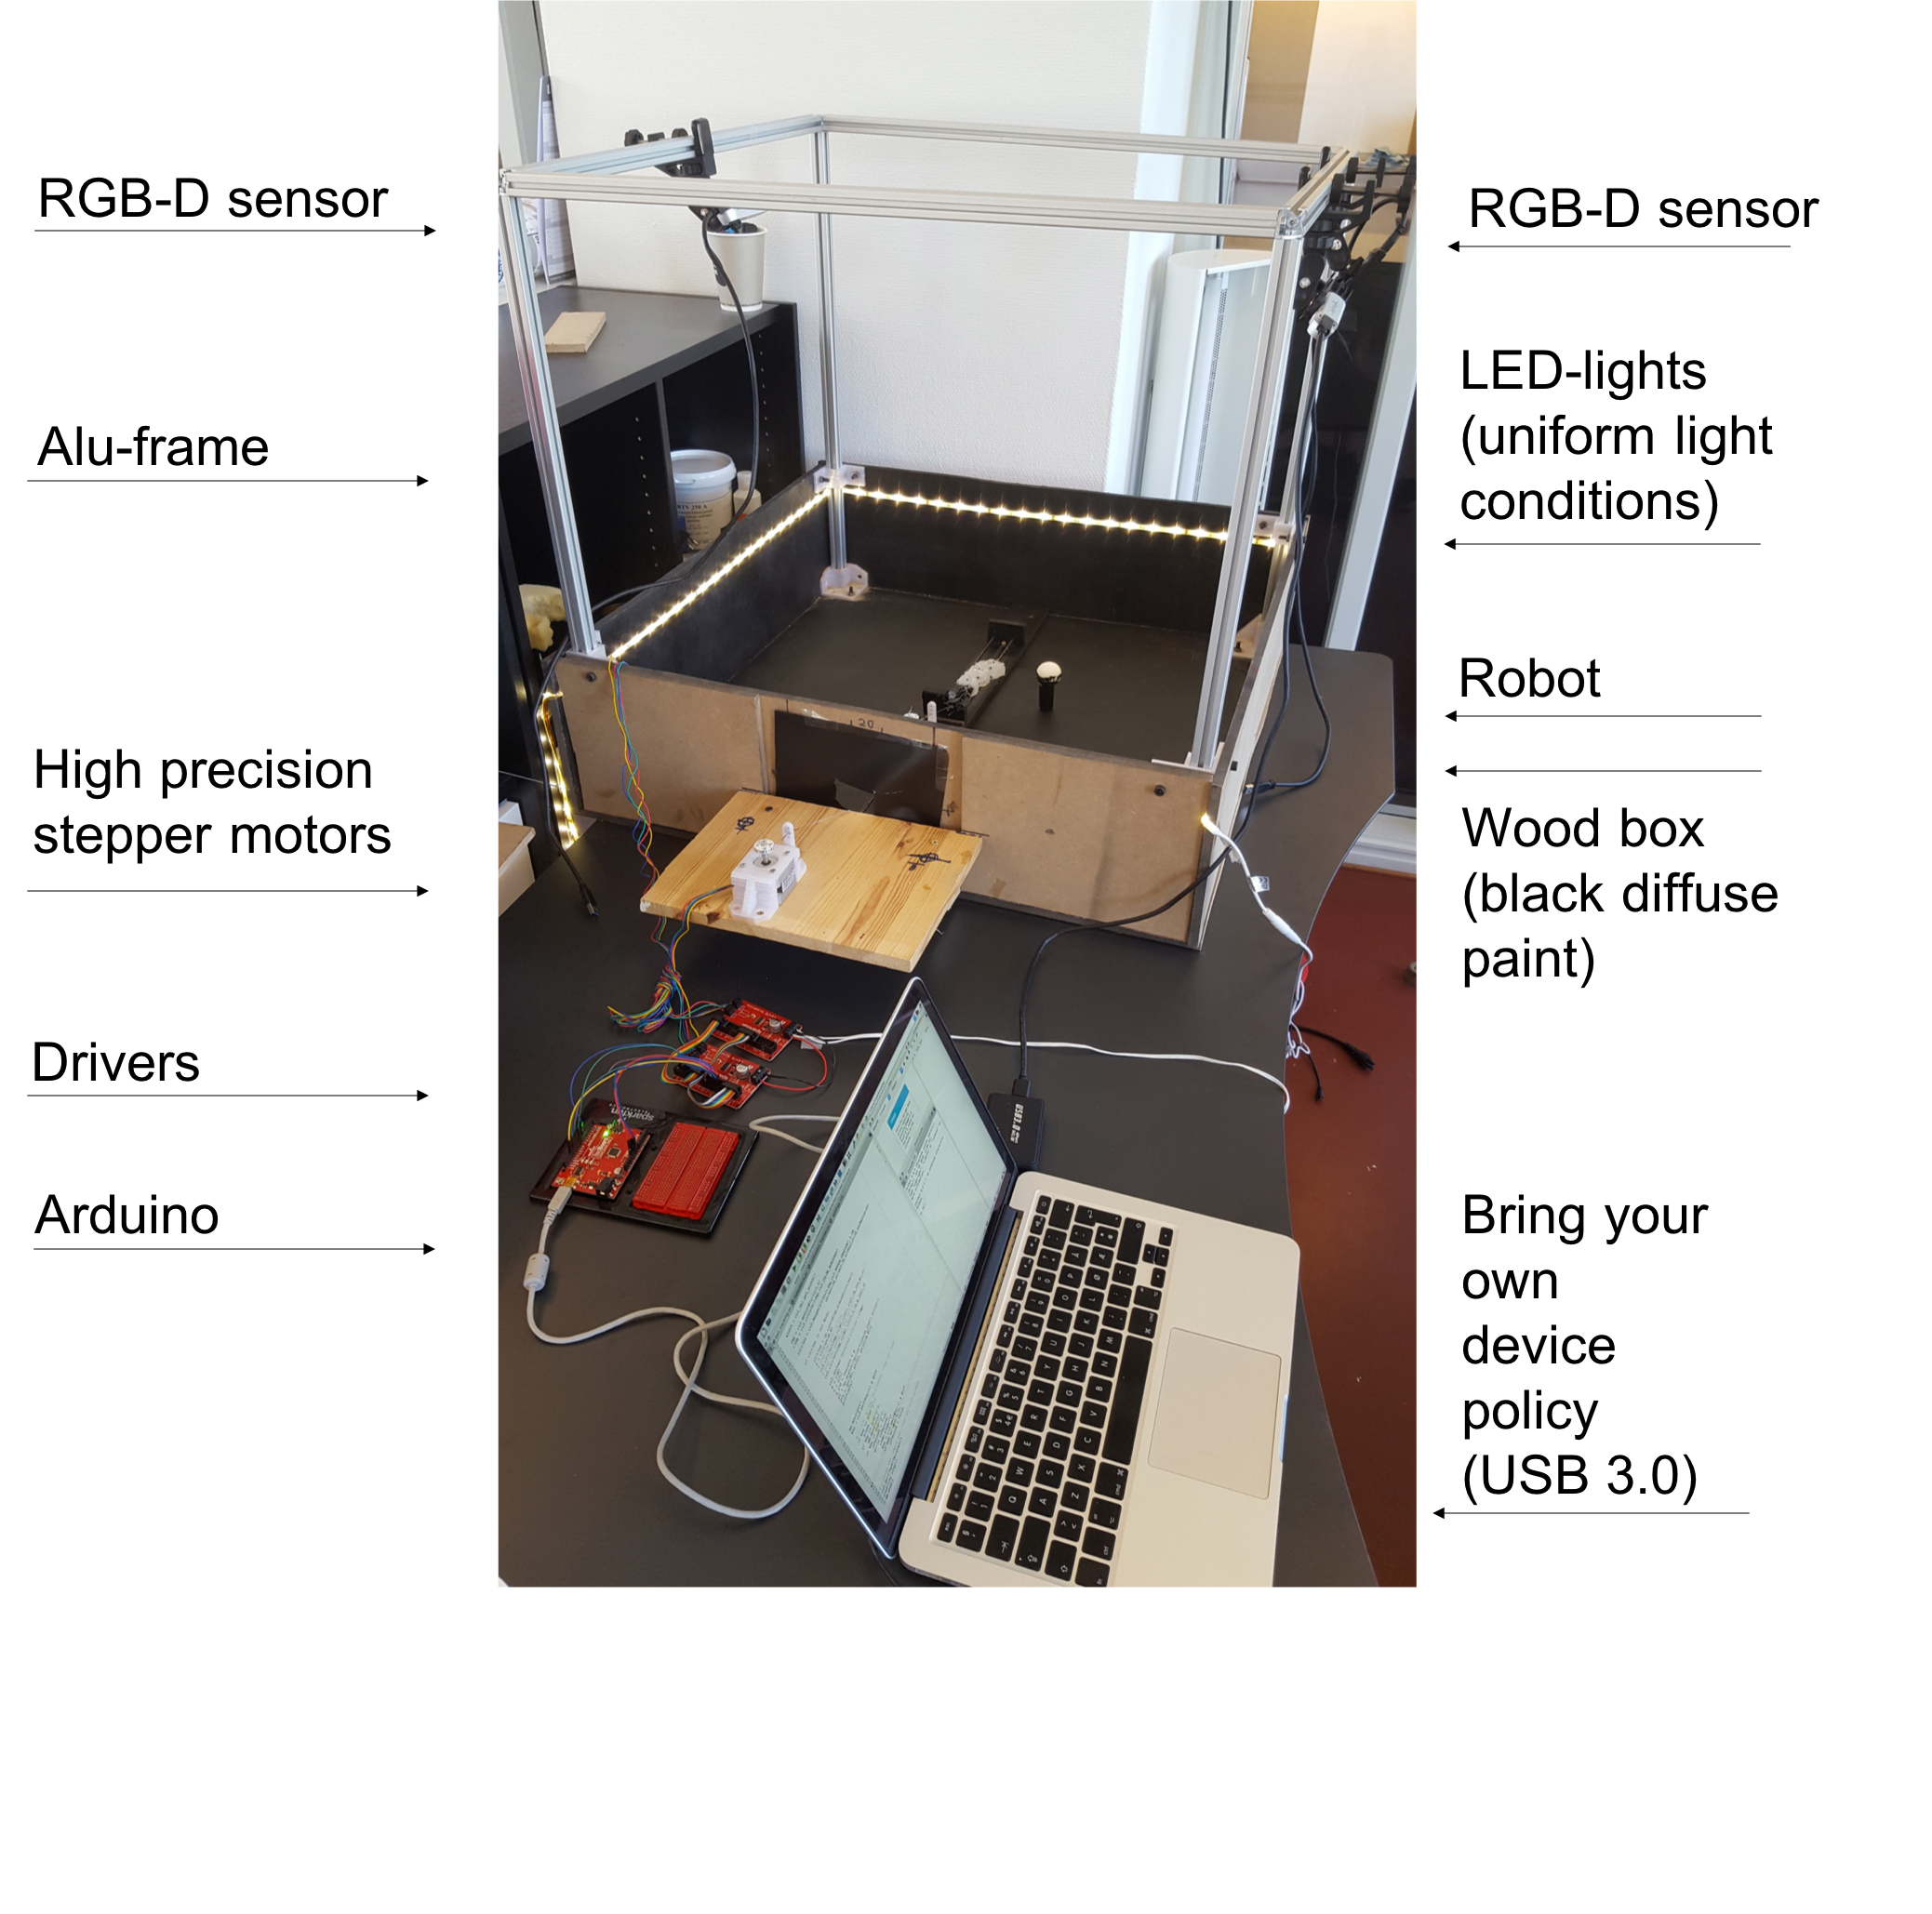
\includegraphics[width=3in,trim={0 5cm 0 0},clip]{figures/learningCube.png}}}
        \caption{Overview of the LearningCube}
        \label{fig:cube}
\end{figure}
\clearpage

\section{LearningCube}
\begin{figure}[htpb]
      \centering
      \framebox{\parbox{3in}{
        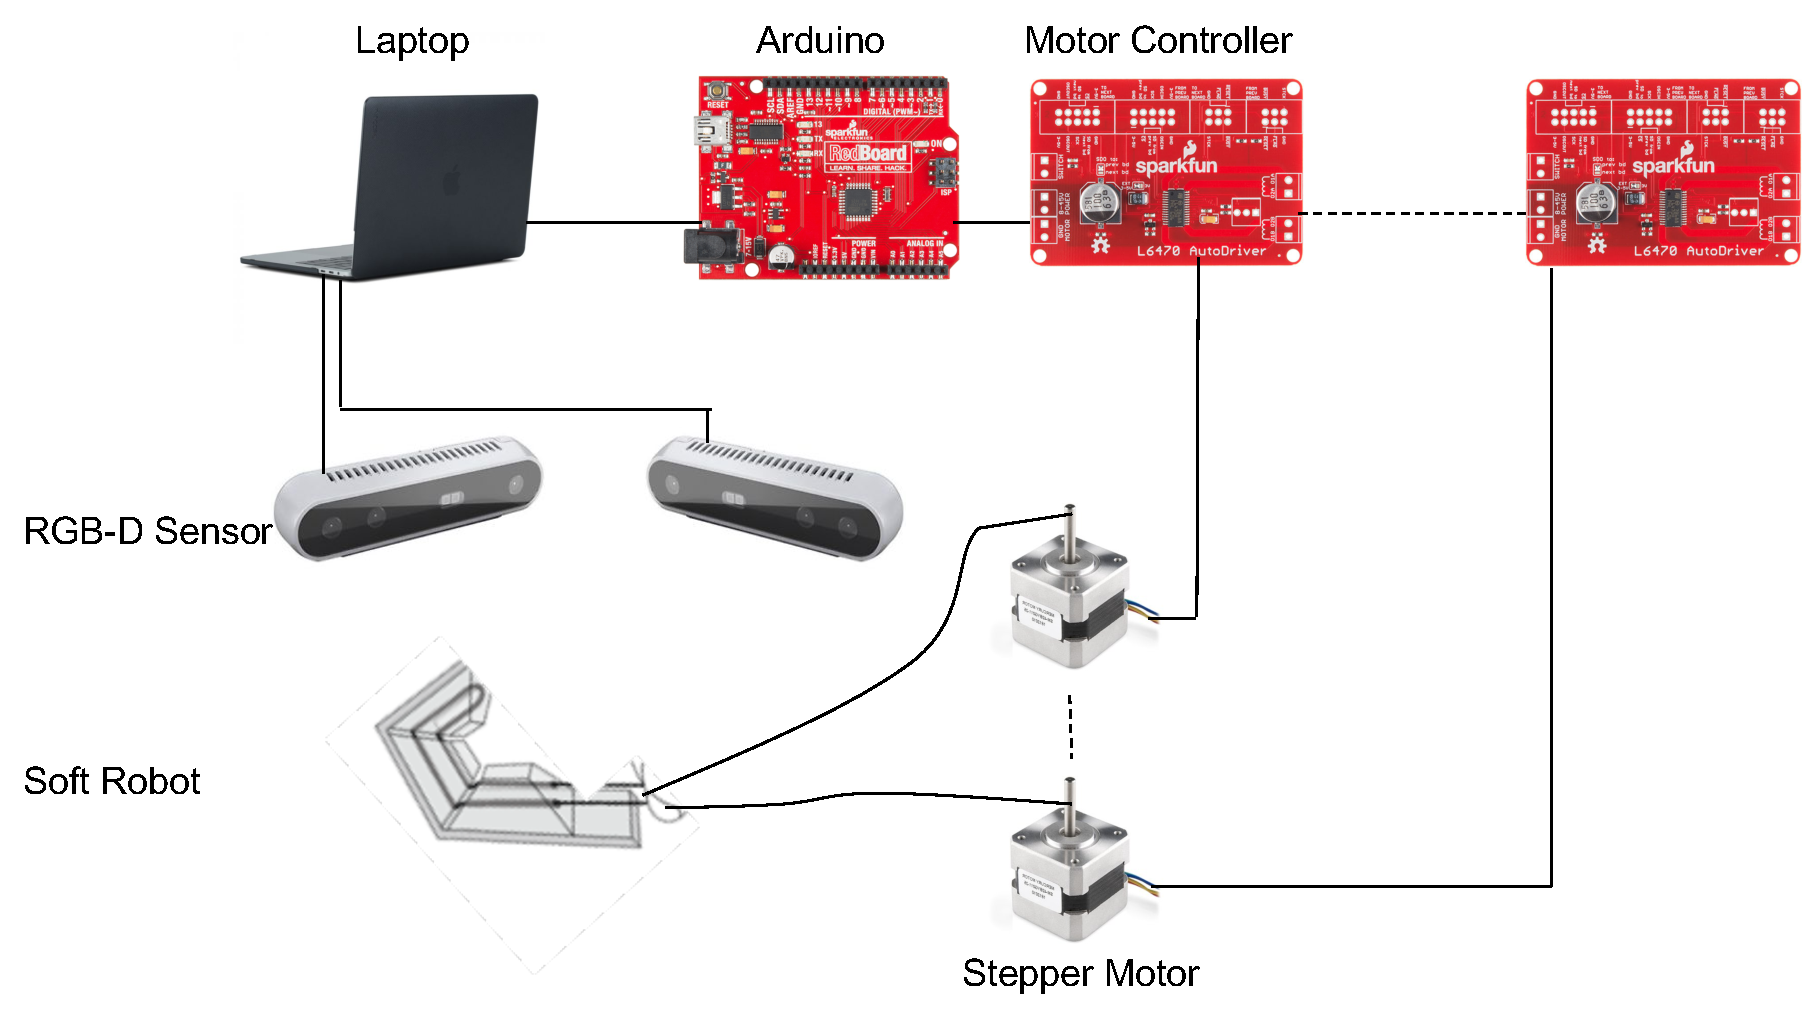
\includegraphics[width=3in]{figures/setup.pdf}}}
        \caption{Sensor and actuator integration}
        \label{fig:setup}
\end{figure}

Since we chose a data driven approach, we need to be able to collect large amounts of high quality data in a reasonable amount of time. We also need a way to interact with the soft robots after we have trained them. Therefore, we first designed and built a platform for data acquisition and experiments. The LearningCube combines depth sensors, motors and robots (see figure \ref{fig:cube}). It consists of a wooden box with aluminum frames. The purpose of the box is to have a rigid base to mount motors and soft robots, but also to block out light pollution and other sources of external noise. Uniform light conditions are provided by LED-strips on all walls. To make segmentation of RGB-D data easy, the base of the box is painted in diffuse black. The aluminum frame lets us mount the cameras almost anywhere without obstructing, which is important for the data quality. 

To control the cable driven soft robots, we need to be able to accurately control the length of the cables. For this purpose, we use 2-phase mercury stepper motors with 1.8 degree steps. The radius of the motor shaft is 2 mm, so one revolution will tighten/loosen the cable by 12.5 mm and one step only by 0.06 mm. Each motor is connected to a stepper motor driver that is used to control speed, acceleration and absolute position of the shaft. The motor drivers are daisy chained to an Arduino, which makes creating a setup with multiple motors easy. We use Intel's RealsSense D415 sensors to capture depth and colour data. Figure \ref{fig:setup} depicts how the Arduino and the depth sensors are integrated in the LearningCube. 

During the training phase, the robots are equipped with visual markers. For each configuration, $\vec{\alpha}$, we want to extract a shape vector from these markers. This is done by segmenting visual markers from the colour images and extracting the corresponding x,y,z coordinates from the point cloud. The result is a shape vector (see figure \ref{fig:shape}).

A point cloud generated from a depth sensor can only contain points on the surface of the object that is visible for the sensor. One can, however, make a more complete reconstruction of the object by merging point clouds from several sensors with different viewpoints. Under the assumption that noise and degradation is negligible, two corresponding points, as seen from two sensors, are related by a rigid transformation. The translation and rotation can be found by least squares fitting of control points from each coordinate system (CITE). As control points, we use detected centroids of fuss-balls, due to high production quality and equal appearance from all angles (see figure \ref{fig:ball}). 
Point correspondences between points in the respective coordinate systems have to, however, be determined before applying the least squares method. This is done by searching for the permutation of detected points in coordinate system B, as:
$$
    \pi^* = \arg \min_{\pi} \frac{1}{N}\sum_{i=1}^N \|p^A_n- (R(\pi)p^B_{\pi(n)} + T(\pi))\|^2
$$
where ($R(\pi), T(\pi))$ is the rigid transformation between $p^A $ and $p^B_{\pi}$.

After extracting a shape vector from each sensor, we merge them such that visual markers that are represented in both shape vectors are averaged out. Markers that are common to both sensors are detected by a lower threshold on pairwise marker-distance (see figure \ref{fig:two}).

This process is repeated for each configuration in the sampling space and for each sampled configuration, k, we get a set of points, $p^k$. The points in $p^k$ are not in any particular order, which means that there is no guarantee that $p_i^k$ and $p_i^{k+1}$ refer to the same physical marker. Moreover, the size of the points sets may differ from configuration to configuration due to erroneous segmentation or noise in the depth data. This is solved by sorting all point sets from configurations $k=(2,3,...,K)$ with respect to the order of the first point set $p^1$. This is done by greedily linking markers with the smallest displacement. Missing values are approximated as a gaussian weighted mean of nearby marker displacements and false positives are detected as frequently approximated markers. 

\begin{figure}[htpb]
      \centering
      \framebox{\parbox{3in}{
        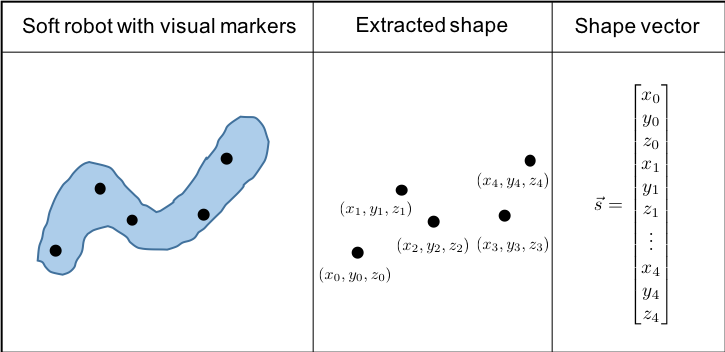
\includegraphics[width=3in]{figures/postiver.png}}}
        \caption{Shape representation of soft robot}
        \label{fig:shape}
\end{figure}

 \begin{figure}[htpb]
        \centering
        \framebox{\parbox{3in}{
        \begin{subfigure}[b]{1.4in} 
                \centering
                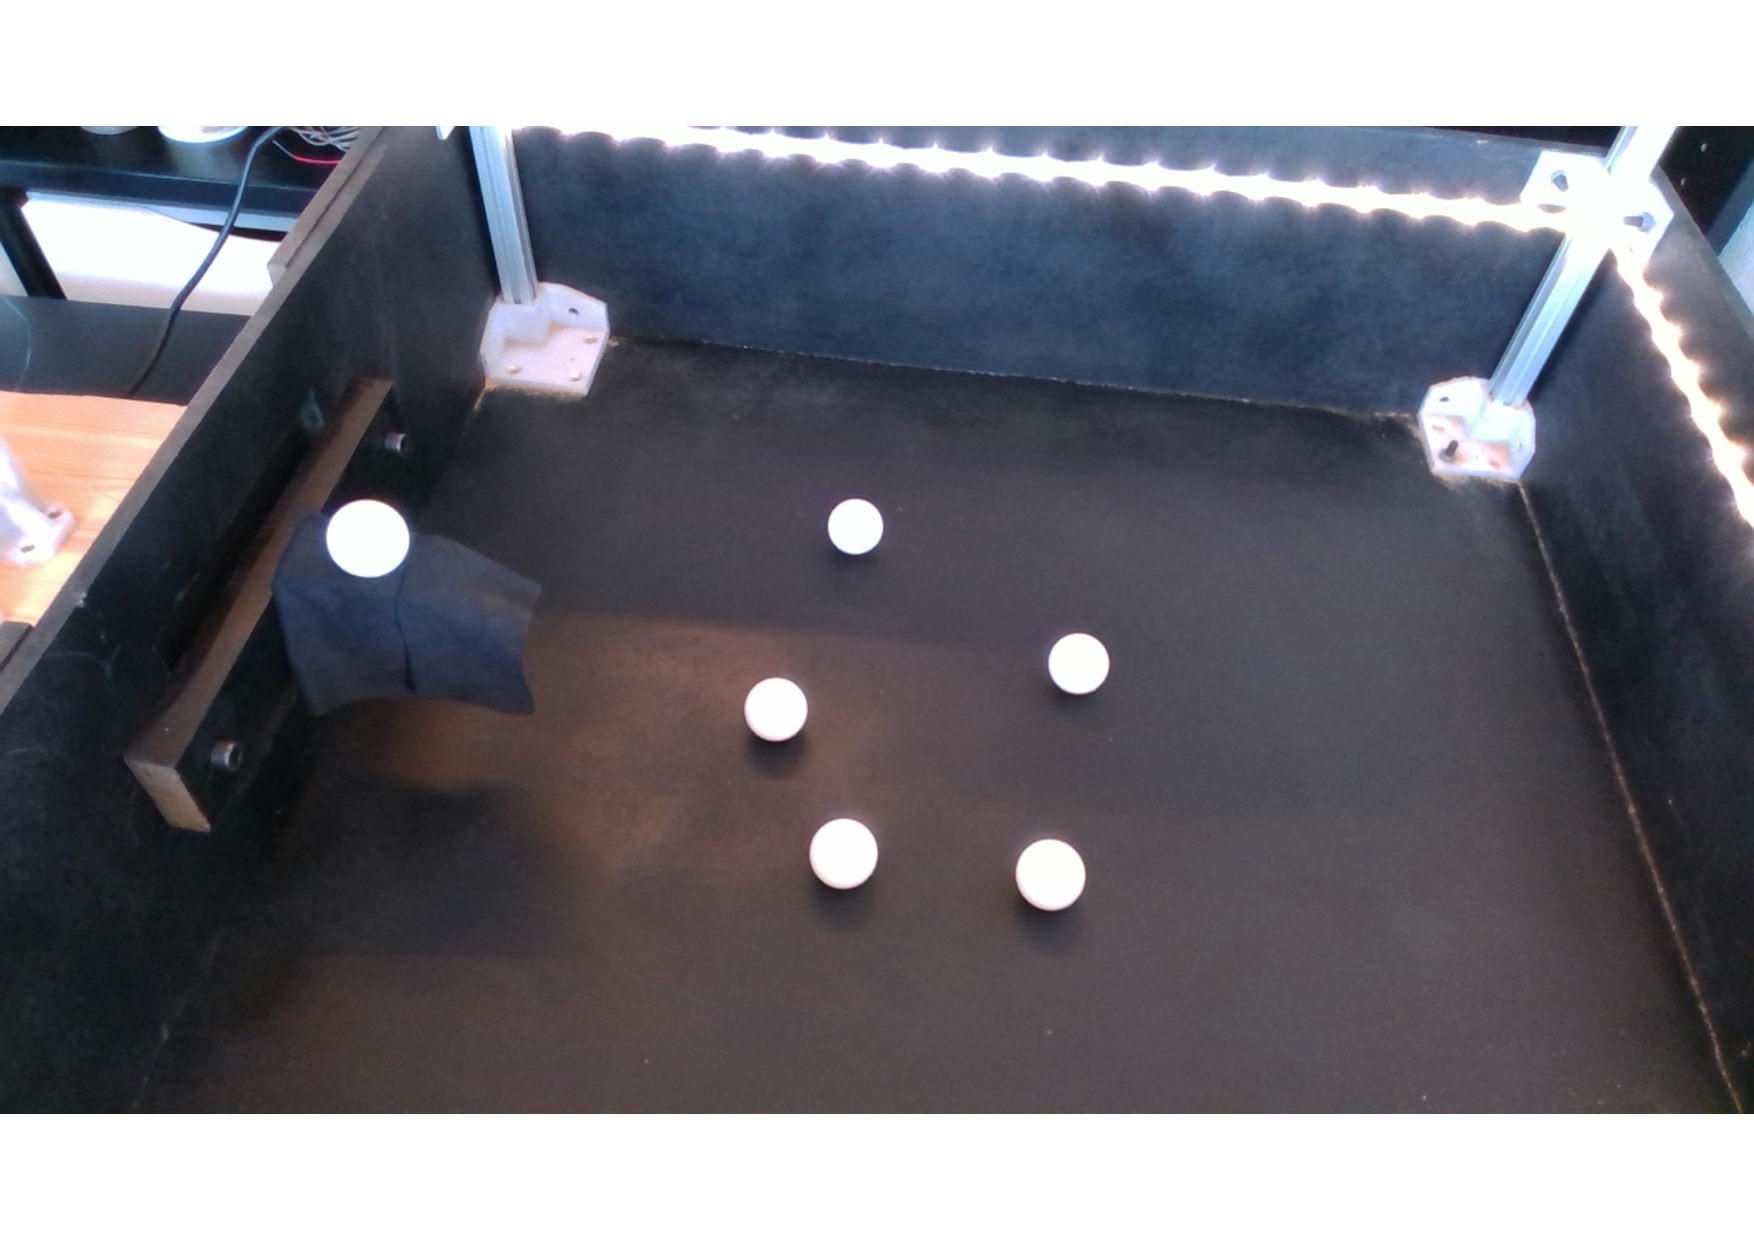
\includegraphics[width=\textwidth]{figures/calib1.pdf}
        \end{subfigure}
        \begin{subfigure}[b]{1.4in}                            
                \centering
                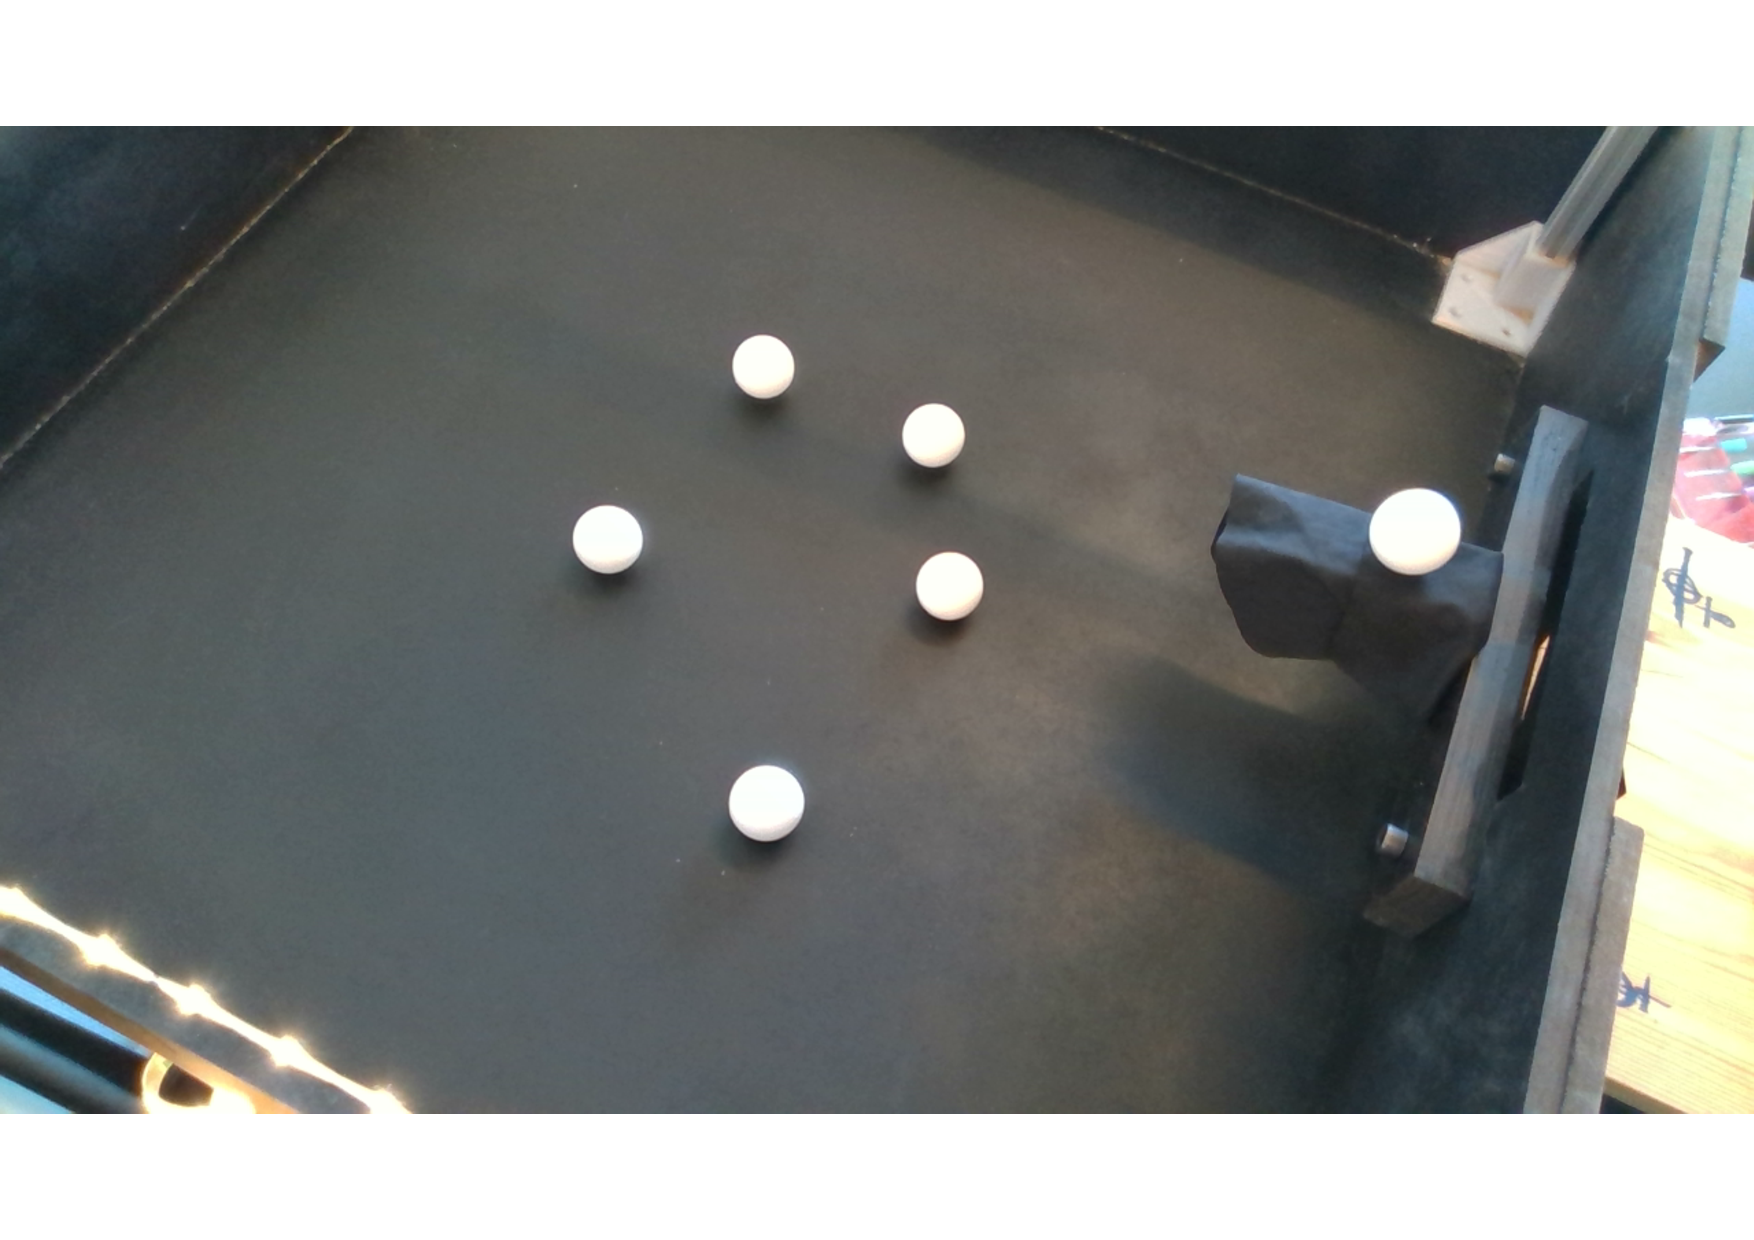
\includegraphics[width=\textwidth]{figures/calib2.pdf}
        \end{subfigure}}}
        \caption{Calibration balls seen from two sensors}
        \label{fig:ball}
\end{figure}

 \begin{figure}[htpb]
        \centering
        \framebox{\parbox{3in}{
        \begin{subfigure}[b]{1.4in} 
                \centering
                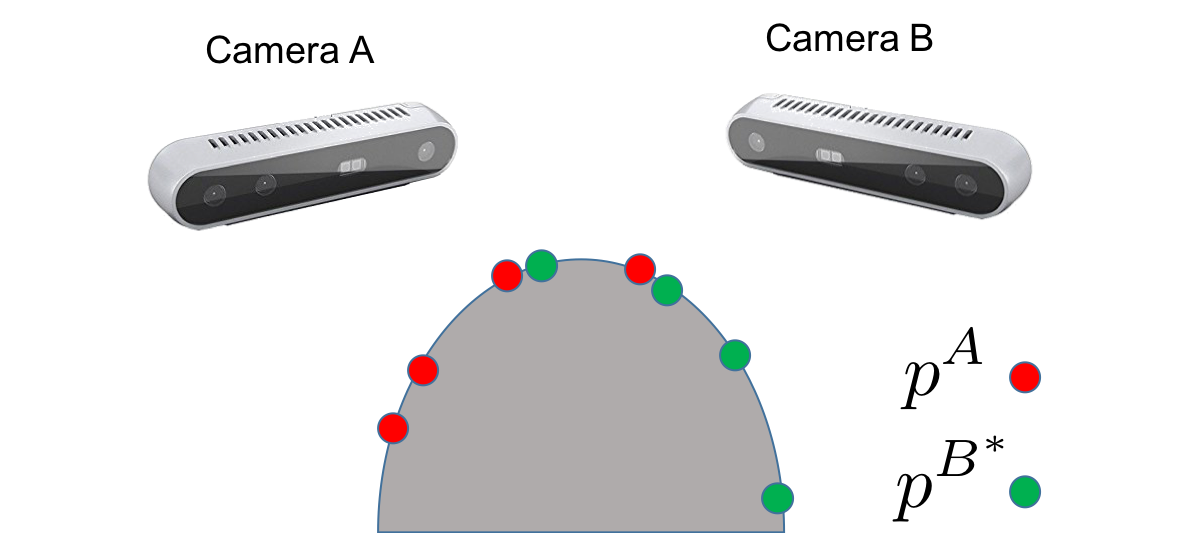
\includegraphics[width=\textwidth]{figures/common2.png}
        \end{subfigure}
        \begin{subfigure}[b]{1.4in}                            
                \centering
                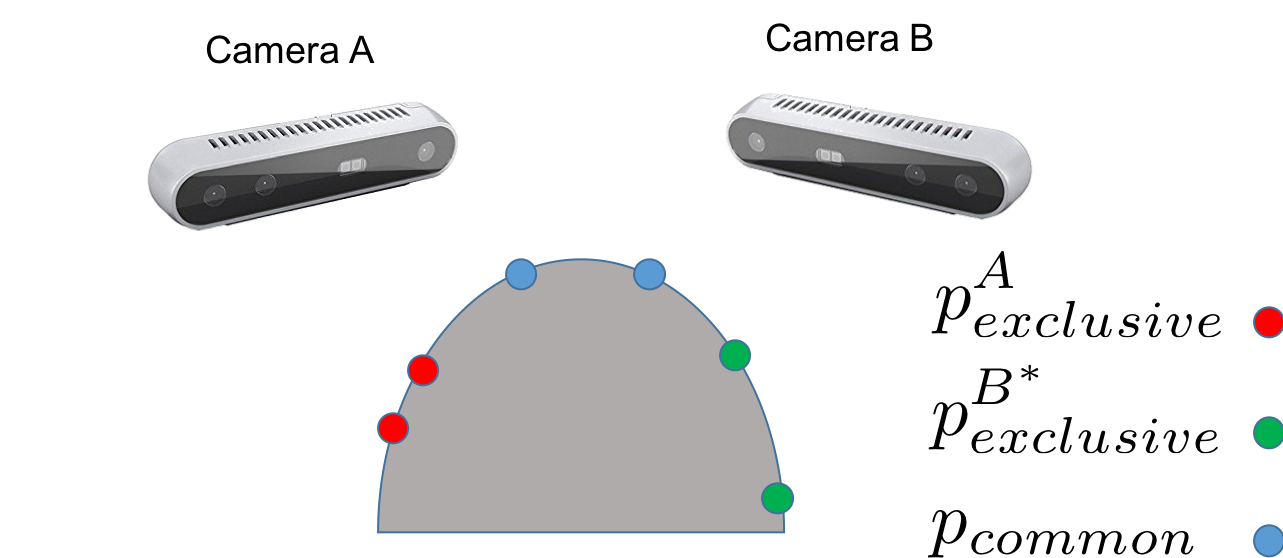
\includegraphics[width=\textwidth]{figures/common1.png}
        \end{subfigure}}}
        \caption{Common markers taken into account}
        \label{fig:two}
\end{figure}

\clearpage
   
\section{Data Driven Inverse Kinematics for Soft Robots}
\blindtext[2]
\subsection{Domain Decomposition of Control Space}
\blindtext[2]
 \begin{figure}[htpb]
        \centering
        \framebox{\parbox{3in}{
        \begin{subfigure}[b]{1.4in} 
                \centering
                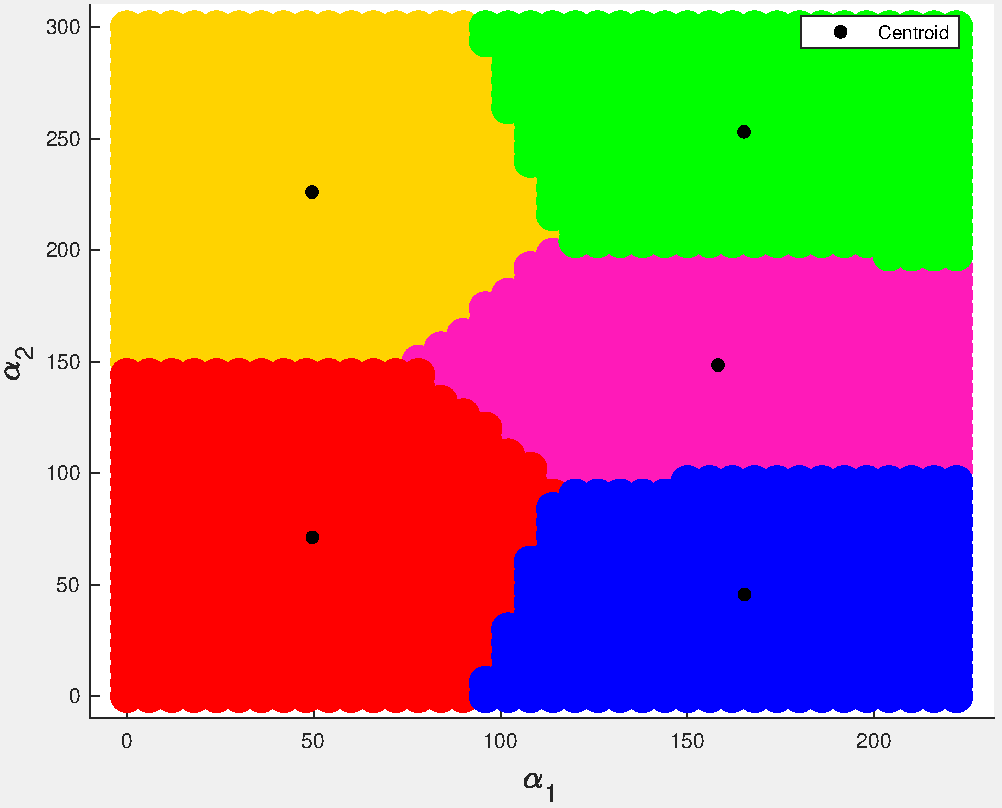
\includegraphics[width=\textwidth]{figures/kmeansseg3.pdf}
        \end{subfigure}
        \begin{subfigure}[b]{1.4in}                            
                \centering
                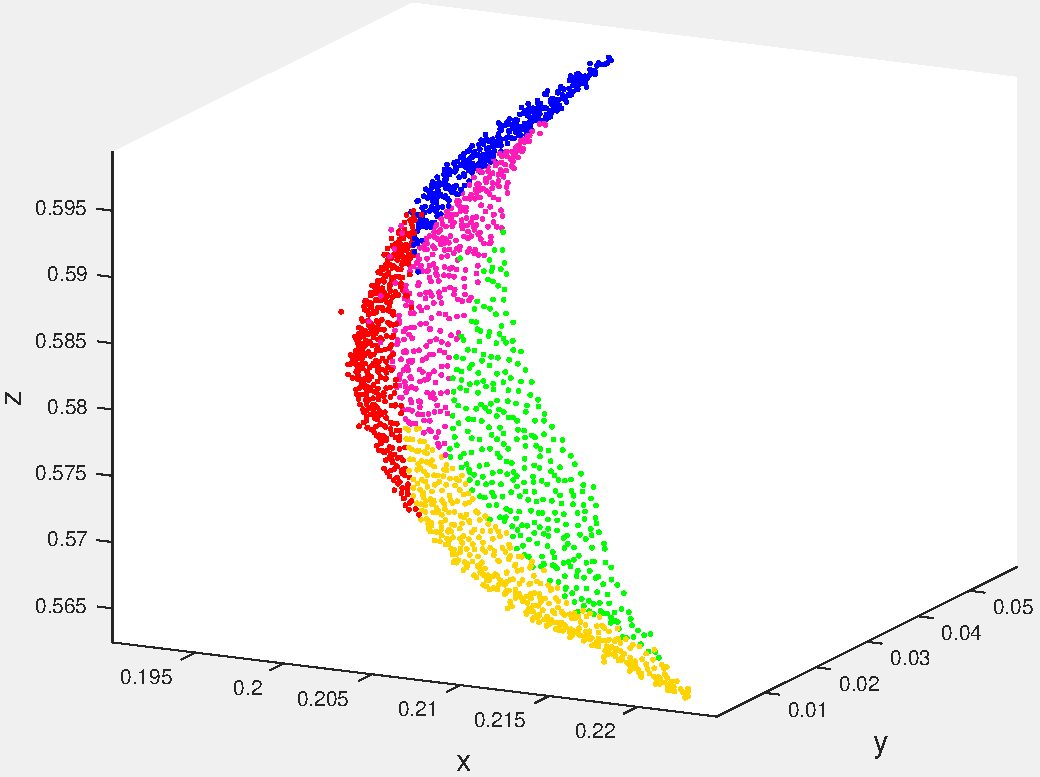
\includegraphics[width=\textwidth]{figures/kmeansseg1.pdf}
        \end{subfigure}}}
        \caption{Calibration balls seen from two sensors}
        \label{fig:calib}
\end{figure}
\blindtext[3]
\subsection{Efficient Polynomial Regression for Higher Order Models}
\blindtext[6]
\begin{figure}[htpb]
      \centering
      \framebox{\parbox{3in}{
        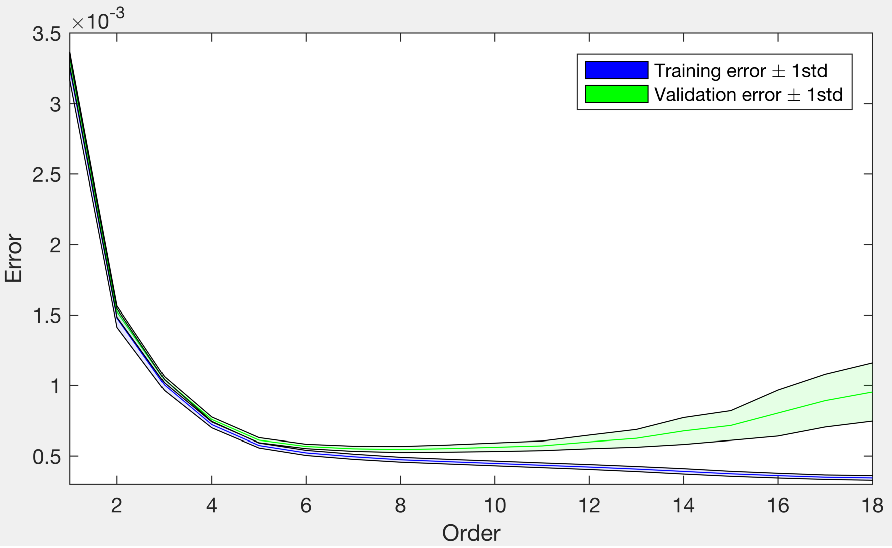
\includegraphics[width=3in]{figures/order_exp.pdf}}}
        \caption{Overview of the LearningCube}
        \label{fig:cube}
\end{figure}
\blindtext[1]
\clearpage

\section{Experiments}

\blindtext[1]
 \begin{figure}[htpb]
        \centering
        \begin{subfigure}[b]{1in} 
                \centering
                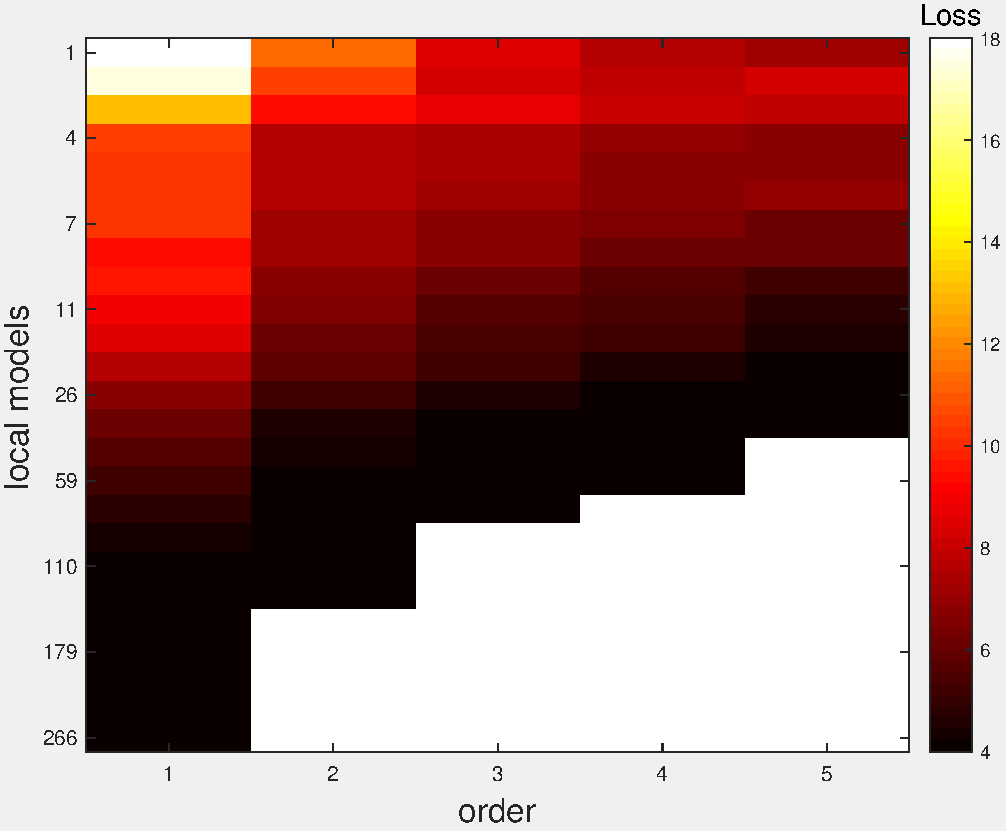
\includegraphics[width=\textwidth]{figures/cross_allQP1.pdf}
                \caption{Training error}
                \label{fig:crossval_train}
        \end{subfigure}
                \begin{subfigure}[b]{1in} 
                \centering
                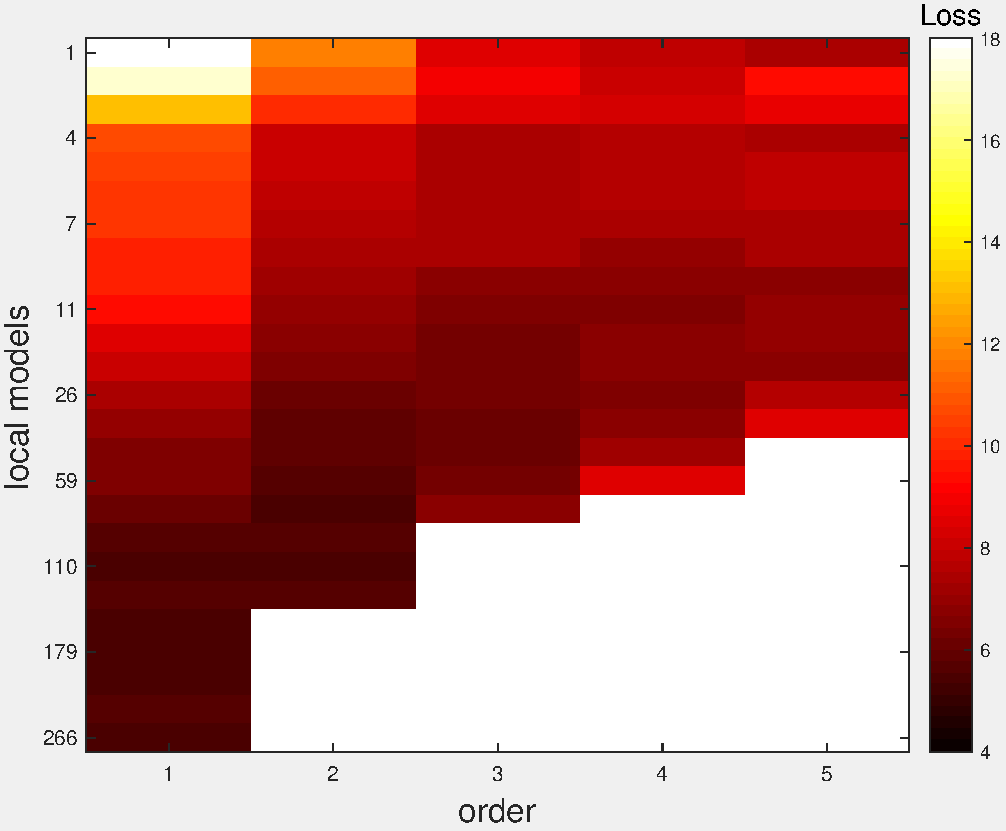
\includegraphics[width=\textwidth]{figures/cross_allQP2.pdf}
                \caption{Validation error}
                \label{fig:crossval_train}
        \end{subfigure}
                \begin{subfigure}[b]{1in} 
                \centering
                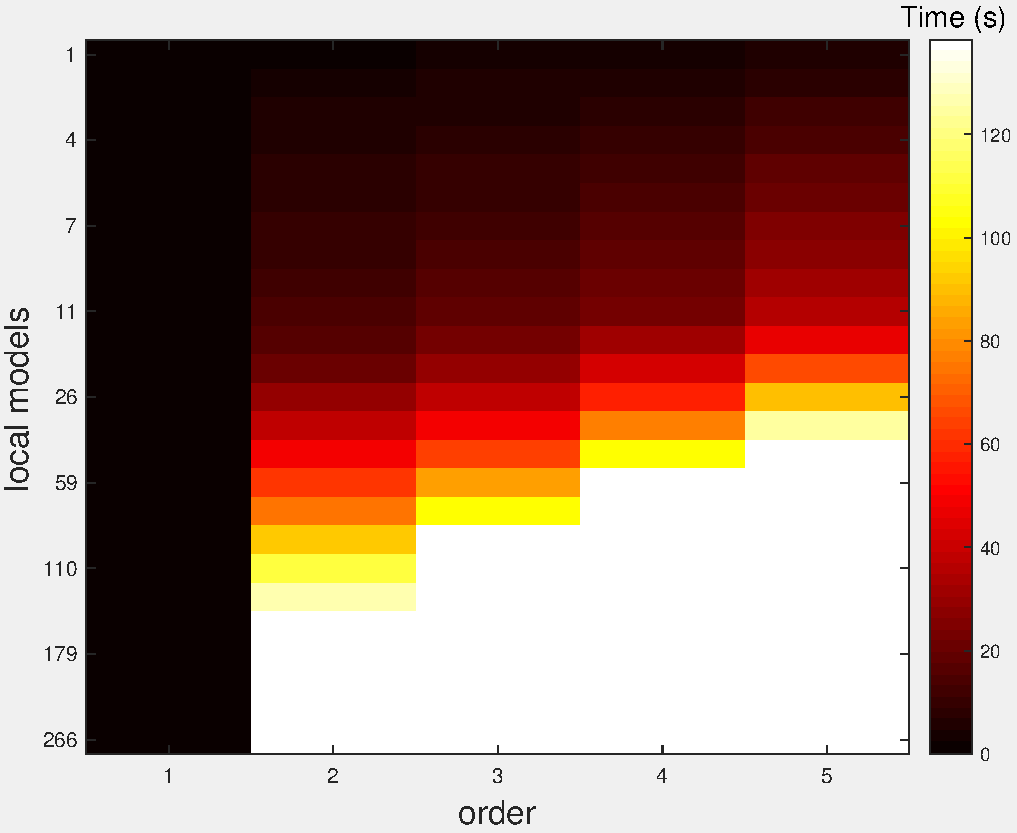
\includegraphics[width=\textwidth]{figures/cross_allQP3.pdf}
                \caption{Execution time}
                \label{fig:crossval_train}
        \end{subfigure}
\end{figure}
\blindtext[1]
 \begin{figure}[htpb]
        \centering
        \begin{subfigure}[b]{1in} 
                \centering
                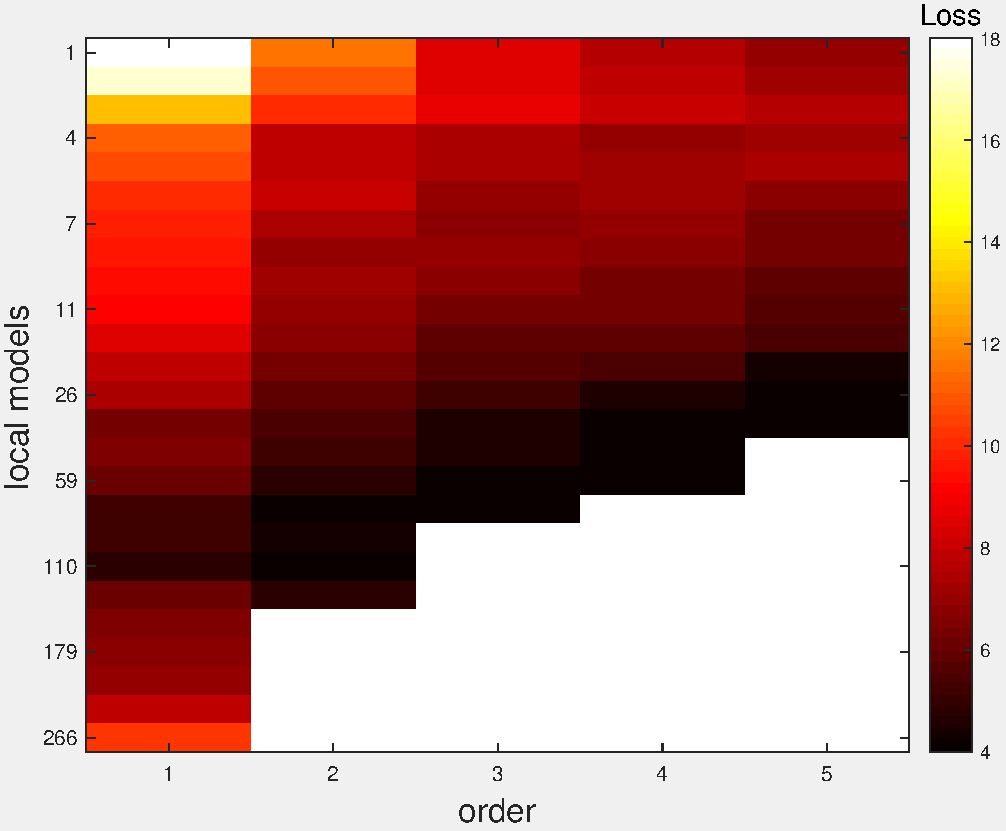
\includegraphics[width=\textwidth]{figures/cross_allreg1.pdf}
                \caption{Training error}
                \label{fig:crossval_train}
        \end{subfigure}
                \begin{subfigure}[b]{1in} 
                \centering
                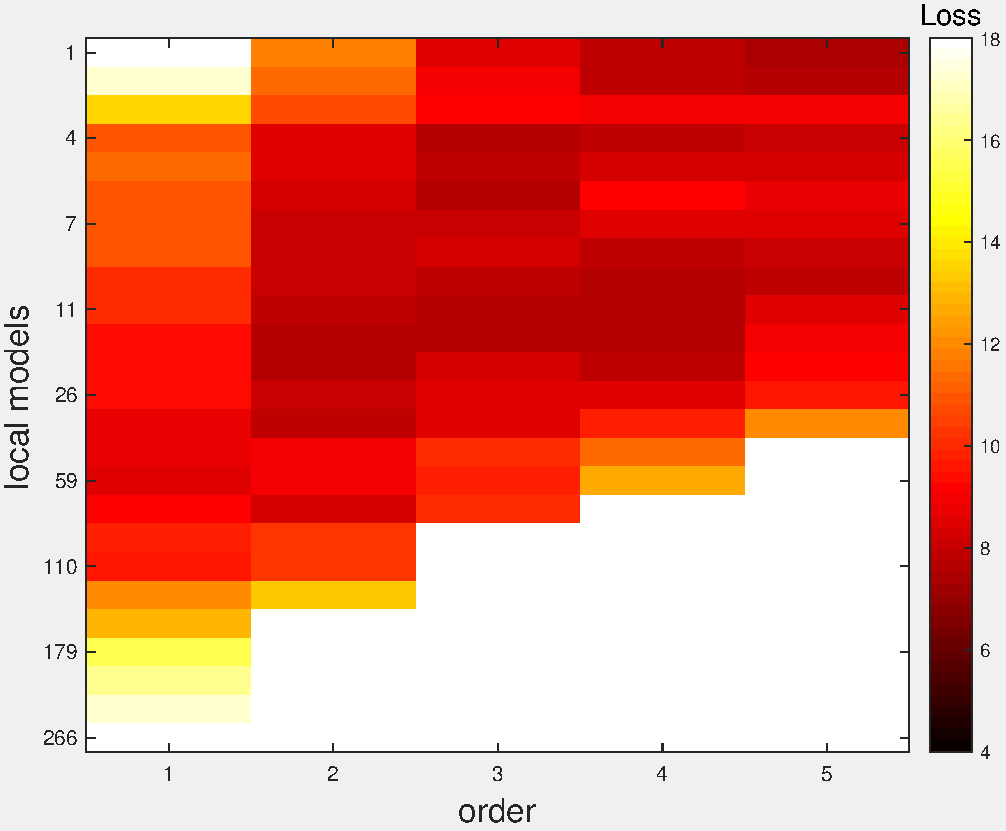
\includegraphics[width=\textwidth]{figures/cross_allreg2.pdf}
                \caption{Validation error}
                \label{fig:crossval_train}
        \end{subfigure}
                \begin{subfigure}[b]{1in} 
                \centering
                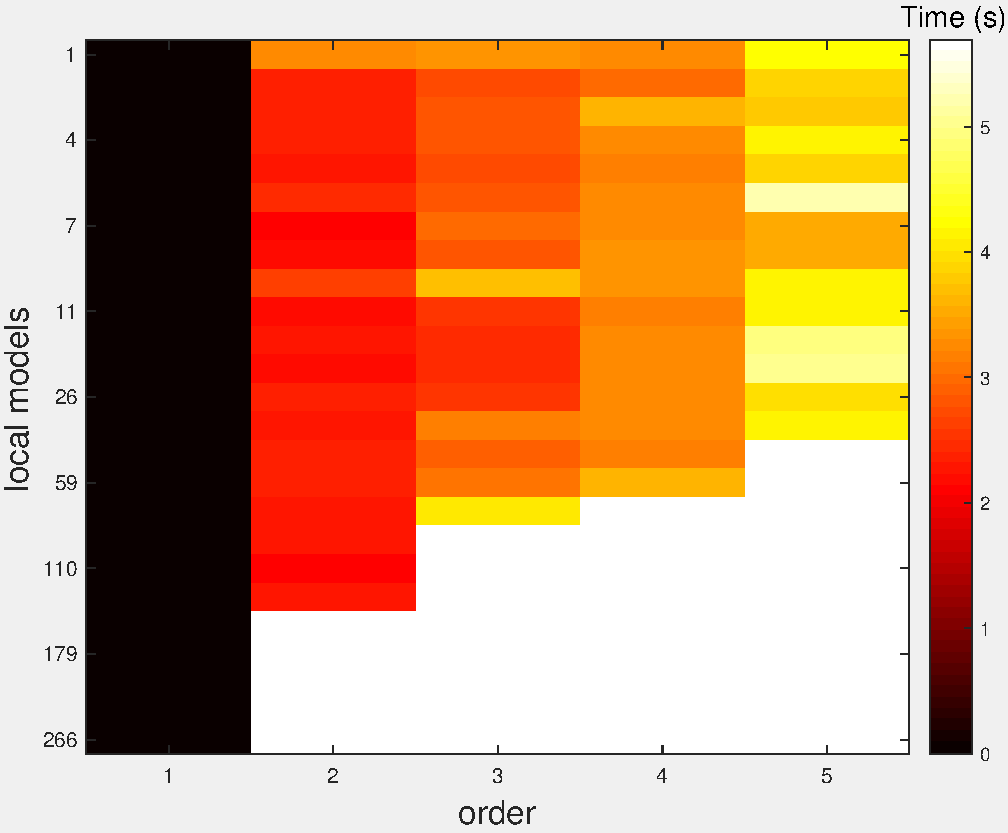
\includegraphics[width=\textwidth]{figures/cross_allreg3.pdf}
                \caption{Execution time}
                \label{fig:crossval_train}
        \end{subfigure}
\end{figure}
\blindtext[1]
 \begin{figure}[htpb]
        \centering
        \begin{subfigure}[b]{0.72in} 
                \centering
                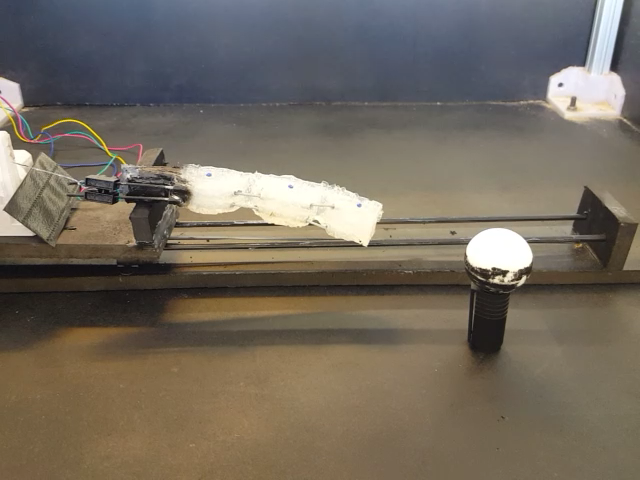
\includegraphics[width=\textwidth]{figures/finger/finger1.png}
        \end{subfigure}
        \begin{subfigure}[b]{0.72in}                            
                \centering
                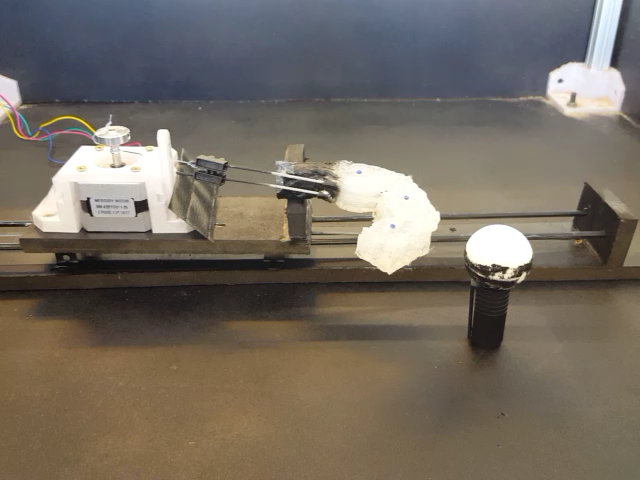
\includegraphics[width=\textwidth]{figures/finger/finger2.png}
        \end{subfigure}
        \begin{subfigure}[b]{0.72in} 
                \centering
                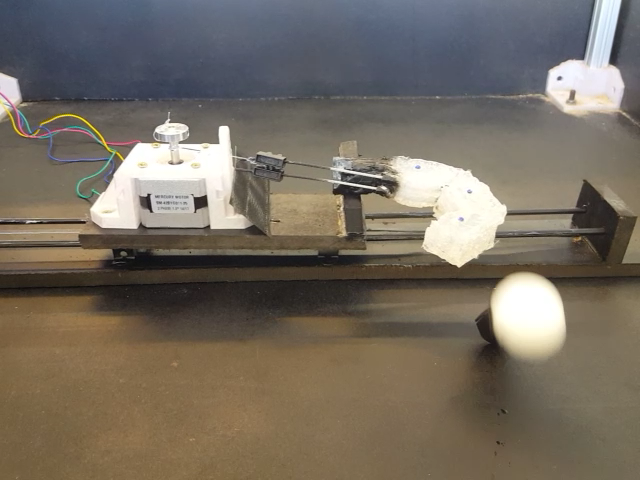
\includegraphics[width=\textwidth]{figures/finger/finger4.png}
        \end{subfigure}
        \begin{subfigure}[b]{0.72in}                            
                \centering
                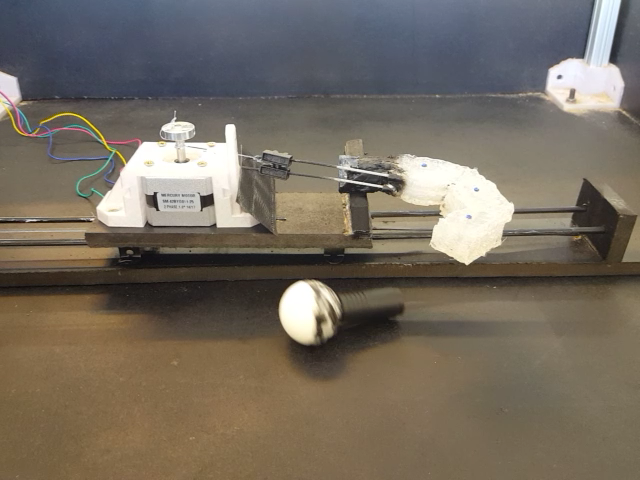
\includegraphics[width=\textwidth]{figures/finger/finger5.png}
        \end{subfigure}
        
        \begin{subfigure}[b]{0.72in} 
                \centering
                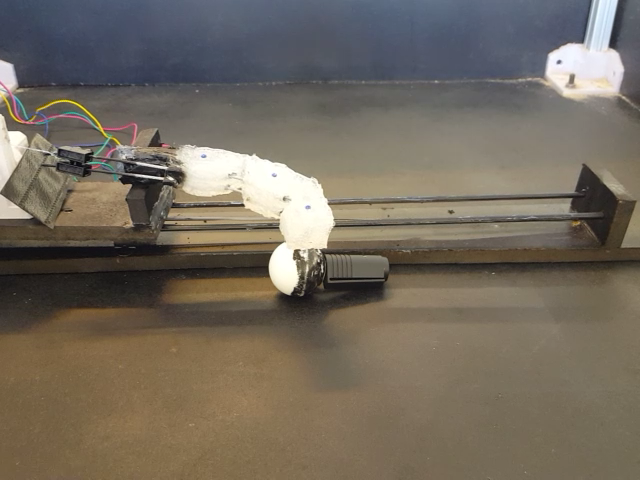
\includegraphics[width=\textwidth]{figures/finger/finger6.png}
        \end{subfigure}
        \begin{subfigure}[b]{0.72in}                            
                \centering
                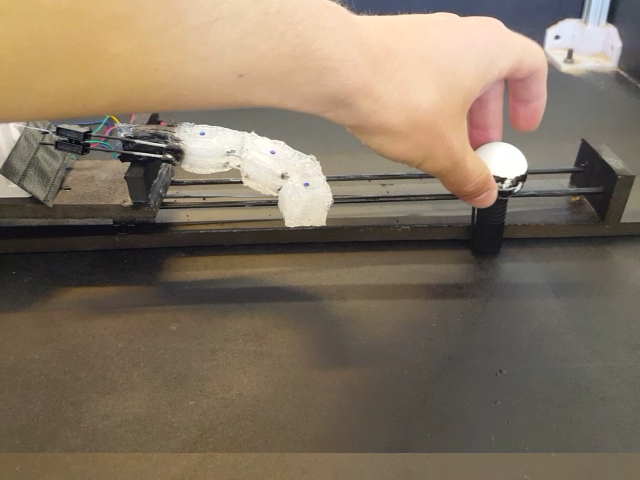
\includegraphics[width=\textwidth]{figures/finger/finger7.png}
        \end{subfigure}
        \begin{subfigure}[b]{0.72in} 
                \centering
                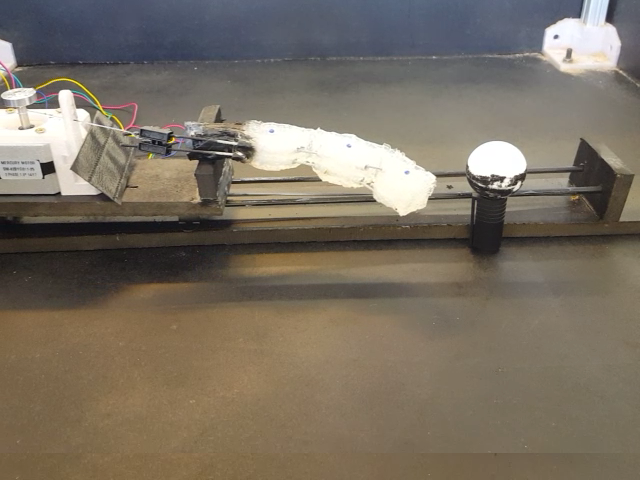
\includegraphics[width=\textwidth]{figures/finger/finger8.png}
        \end{subfigure}
        \begin{subfigure}[b]{0.72in}                            
                \centering
                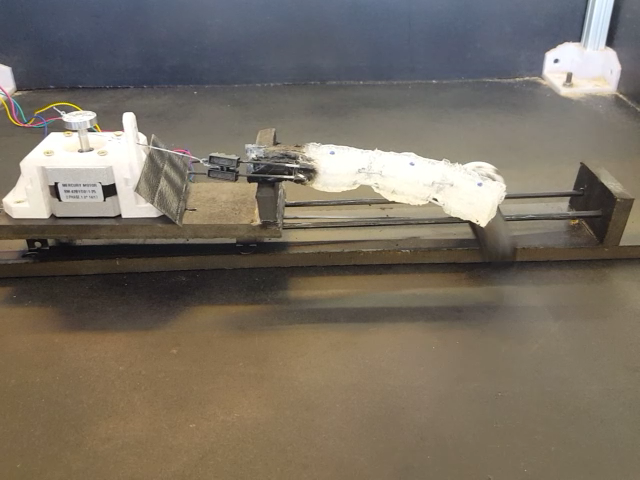
\includegraphics[width=\textwidth]{figures/finger/finger9.png}
        \end{subfigure}
        
        \caption{The finger tries to tip the ball over}
        \label{fig:fingerfun}
        \end{figure}
\blindtext[1]
 \begin{figure}[htpb]
        \centering
        \begin{subfigure}[b]{1.4in} 
                \centering
                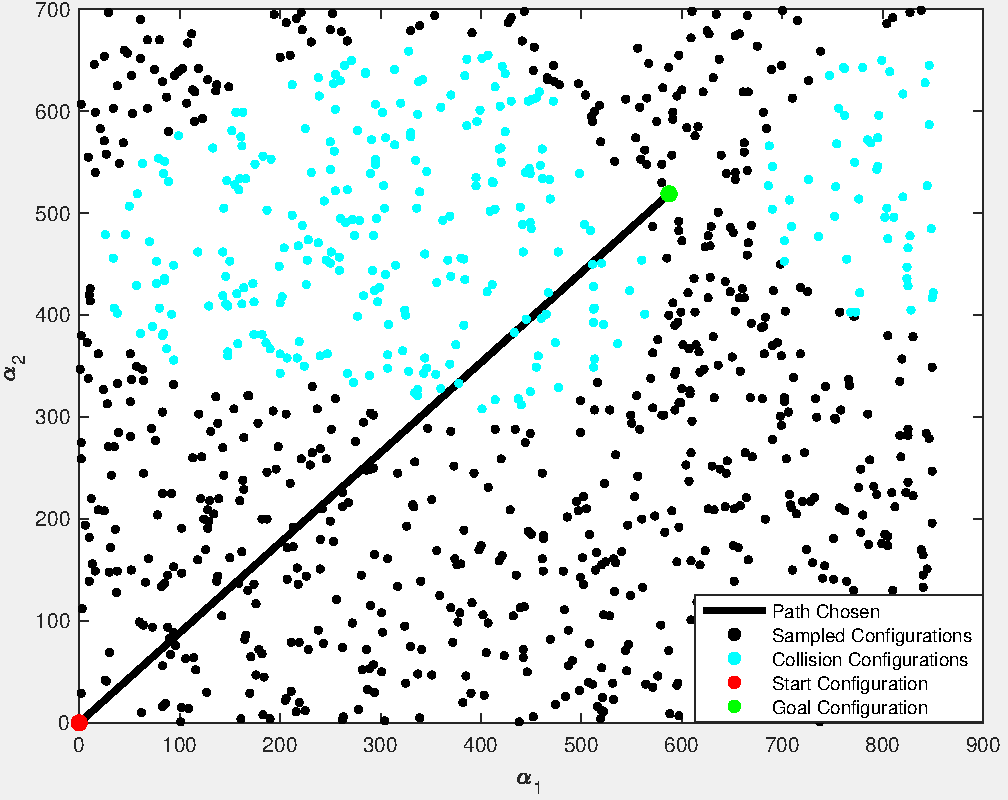
\includegraphics[width=\textwidth]{figures/path/path1.pdf}
                \caption{Naive path}
                \label{fig:path1}
        \end{subfigure}
        \begin{subfigure}[b]{1.4in}                            
                \centering
                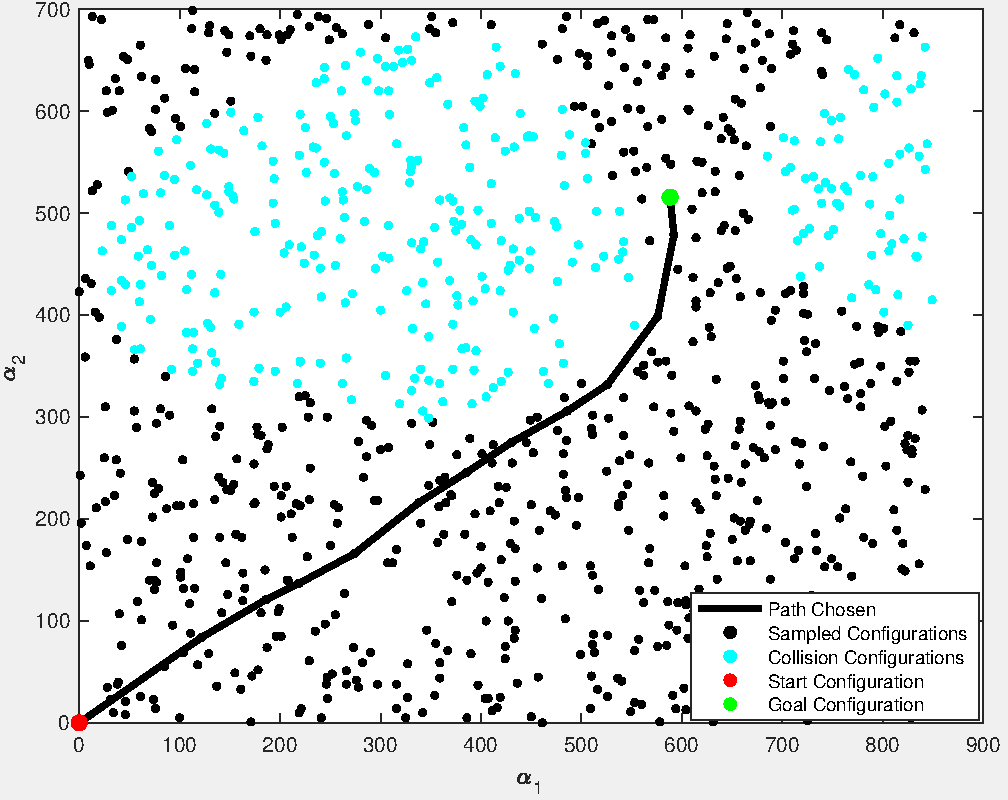
\includegraphics[width=\textwidth]{figures/path/path2.pdf}
                \caption{Collision avoiding path}
                \label{fig:path2}
        \end{subfigure}
        
        \begin{subfigure}[b]{1.4in} 
                \centering
                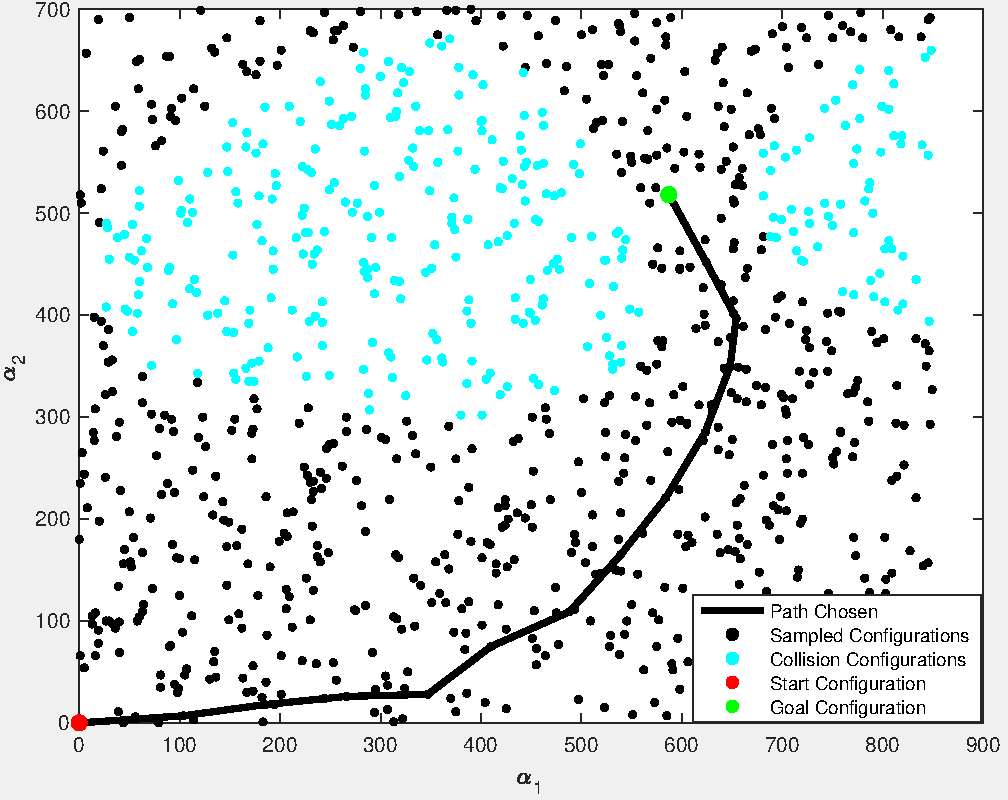
\includegraphics[width=\textwidth]{figures/path/path3.pdf}
                \caption{Minimize probability of collision}
                \label{fig:path3}
        \end{subfigure}
        \begin{subfigure}[b]{1.4in}                            
                \centering
                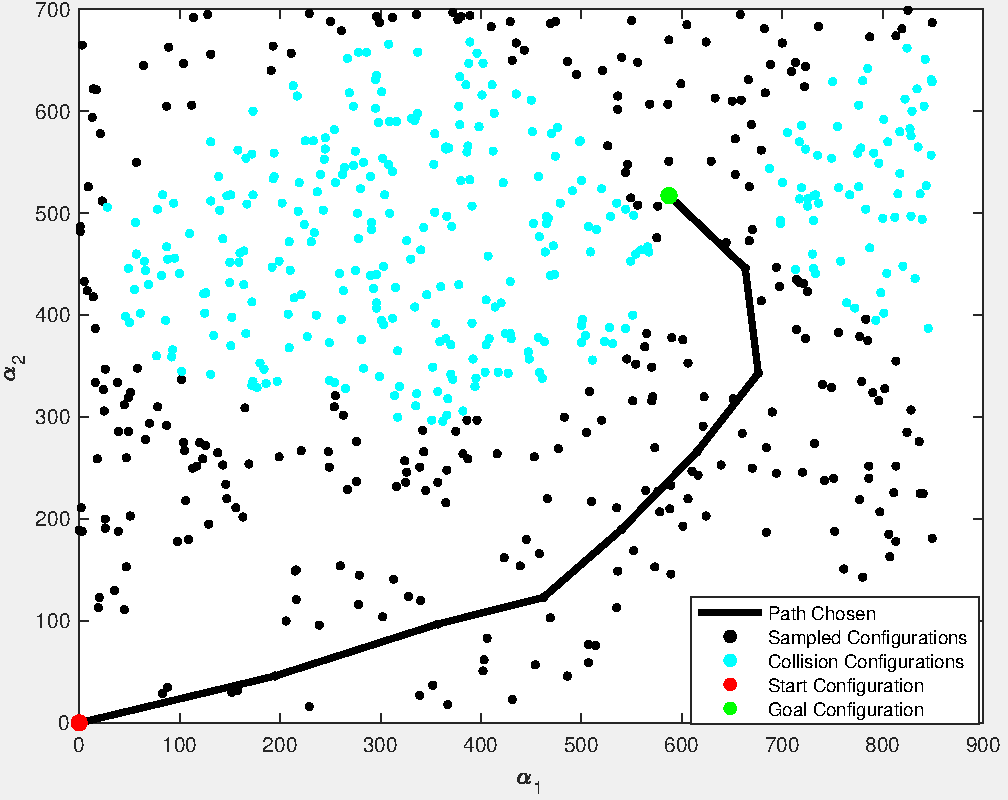
\includegraphics[width=\textwidth]{figures/path/path4.pdf}
                \caption{Importance sampled}
                \label{fig:path4}
        \end{subfigure}
        \caption{Paths through the configuration space}
        \label{fig:path}
\end{figure}

 \begin{figure}[htpb]
        \centering
        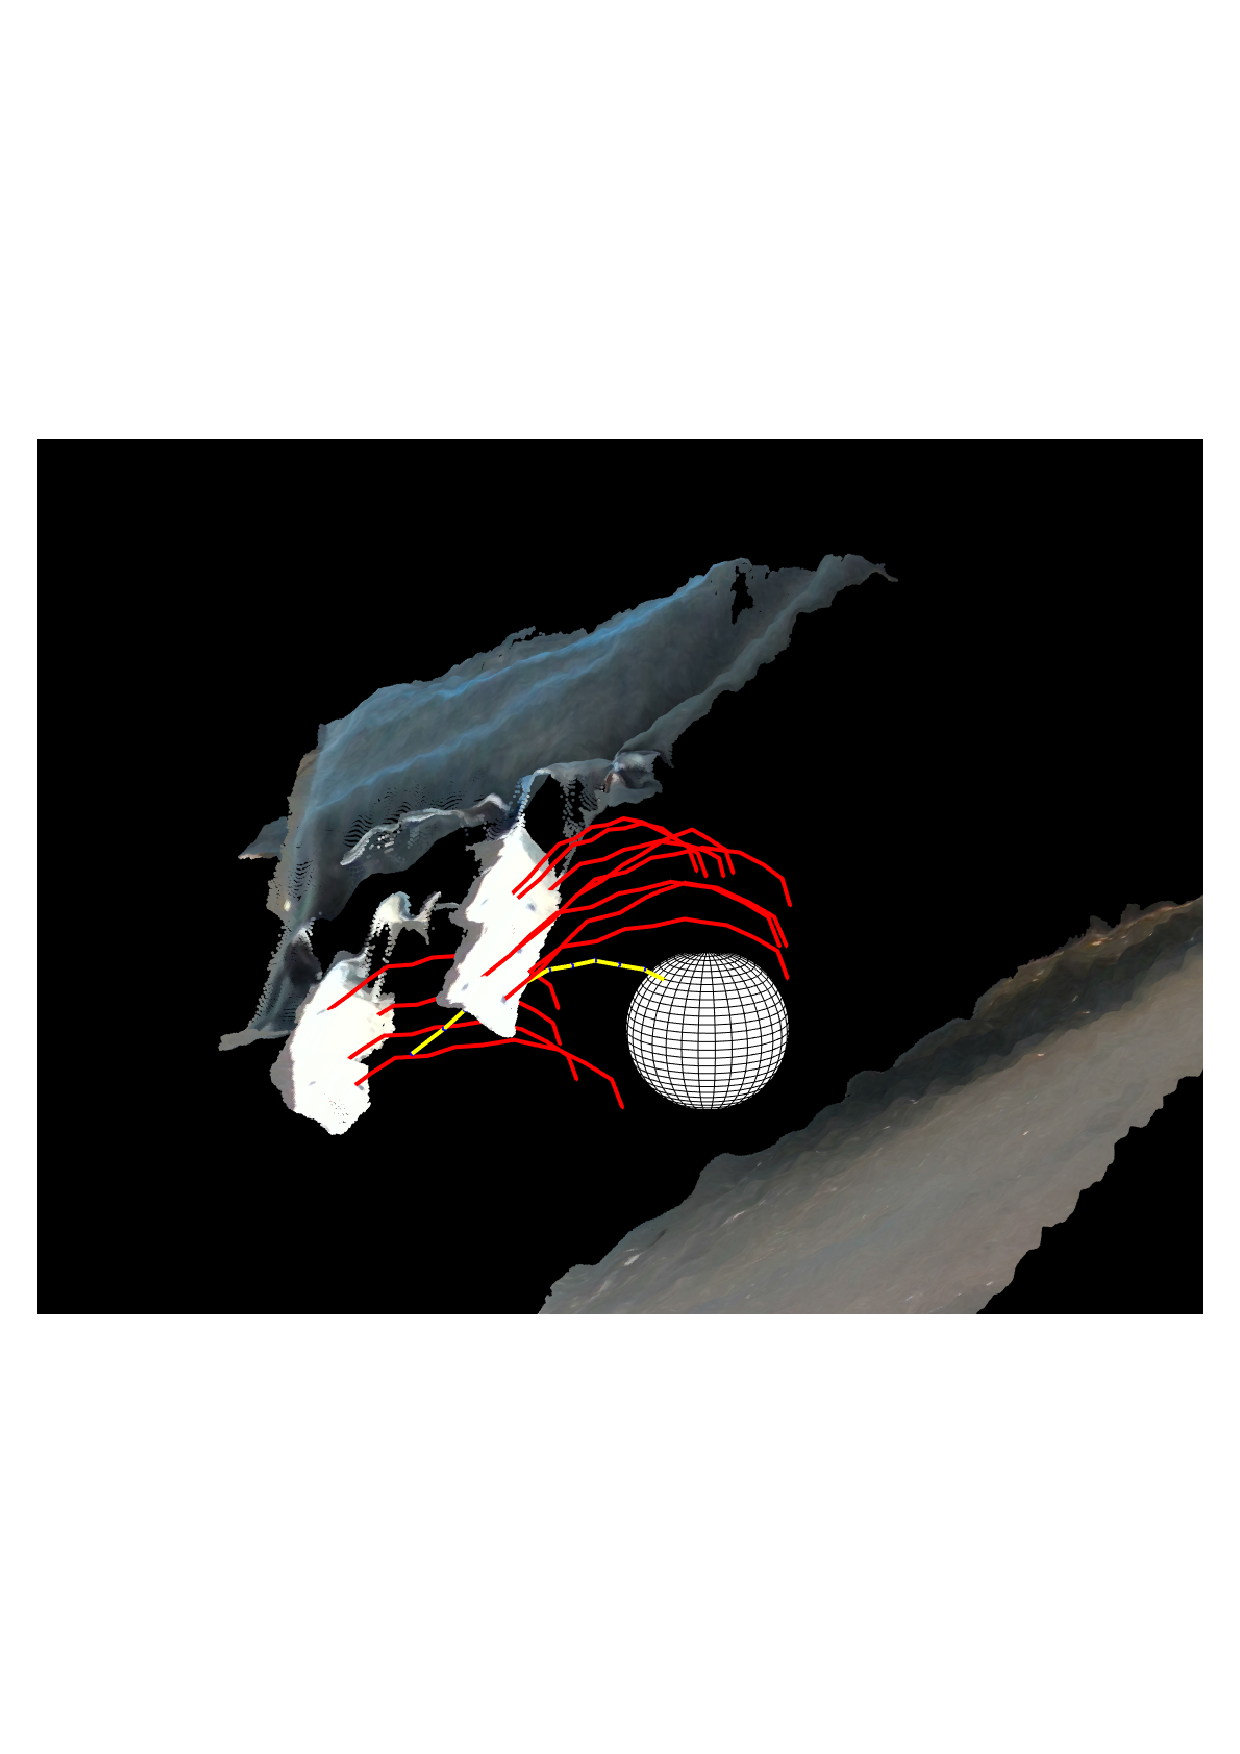
\includegraphics[trim={0 9cm 0 9cm},clip,width=0.5\textwidth]{figures/path/path55.pdf}
        \caption{Trajectory of real markers (red) and phantom marker (yellow) in work-space.}
        \label{fig:work}
\end{figure}

 \begin{figure}[htpb]
        \centering
        \begin{subfigure}[b]{0.72in} 
                \centering
                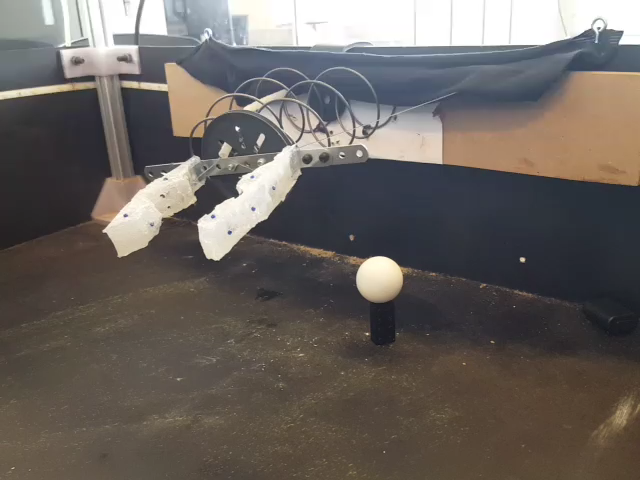
\includegraphics[width=\textwidth]{figures/path/g1.png}
        \end{subfigure}
        \begin{subfigure}[b]{0.72in}                            
                \centering
                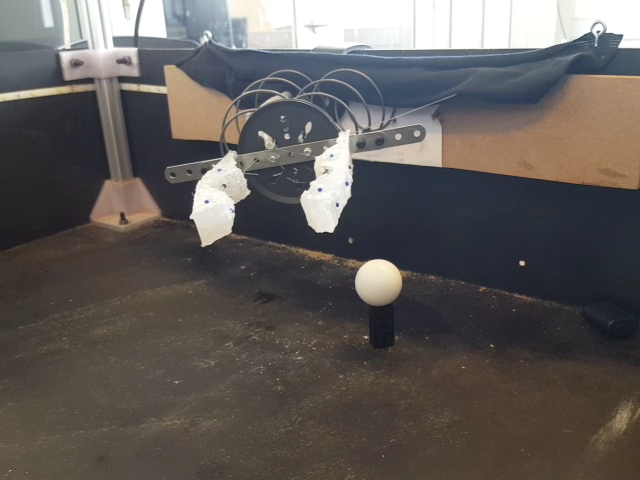
\includegraphics[width=\textwidth]{figures/path/g2.png}
        \end{subfigure}
        \begin{subfigure}[b]{0.72in} 
                \centering
                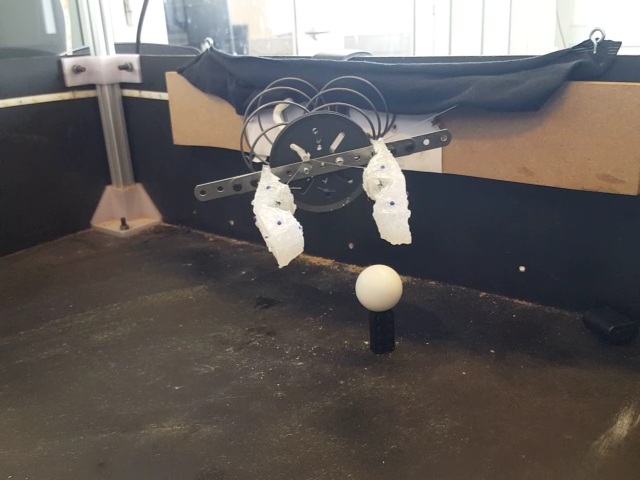
\includegraphics[width=\textwidth]{figures/path/g3.png}
        \end{subfigure}
        \begin{subfigure}[b]{0.72in}                            
                \centering
                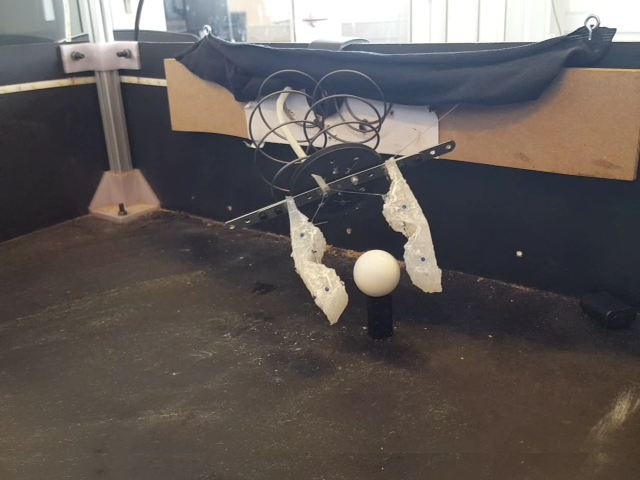
\includegraphics[width=\textwidth]{figures/path/g4.png}
        \end{subfigure}
        \caption{Grabber choosing collision free trajectory}
        \label{fig:grabberpath}
\end{figure}
\blindtext[4]
\section{Discussion and Conclusion}
\blindtext[4]

\addtolength{\textheight}{-12cm}   


\begin{thebibliography}{99}

\bibitem{c1} G. O. Young, ÒSynthetic structure of industrial plastics (Book style with paper title and editor),Ó 	in Plastics, 2nd ed. vol. 3, J. Peters, Ed.  


\end{thebibliography}




\end{document}
